% Lab 02: Reading Markdown Files
% LaTeX Beamer Presentation

\documentclass[aspectratio=169]{beamer}
\usetheme{Madrid}
\usecolortheme{whale}
\setbeamertemplate{navigation symbols}{}
\setbeamertemplate{footline}[frame number]

\usepackage{listings}
\usepackage{graphicx}
\usepackage{tikz}

\lstset{
    language=Python,
    basicstyle=\ttfamily\small,
    keywordstyle=\color{blue}\bfseries,
    stringstyle=\color{red},
    commentstyle=\color{green!60!black},
    showstringspaces=false,
    frame=single,
    backgroundcolor=\color{gray!10},
    breaklines=true
}

\title{Lab 02: Reading Markdown Files}
\subtitle{Loading Documents for RAG Systems}
\author{CSI403 - Full Stack Program Development}
\date{}

\begin{document}

\begin{frame}
    \titlepage
\end{frame}

\begin{frame}{Today's Agenda}
    \begin{columns}
        \begin{column}{0.5\textwidth}
            \textbf{Learning:}
            \begin{itemize}
                \item Why read files?
                \item Opening files in Python
                \item Reading content
                \item Counting and searching
                \item File encoding (UTF-8)
            \end{itemize}
        \end{column}
        \begin{column}{0.5\textwidth}
            \textbf{Time:}
            \begin{itemize}
                \item Lecture: 30 min
                \item Tutorial: 60 min
                \item Break: 15 min
                \item Exercise: 45 min
                \item Submit: 15 min
            \end{itemize}
        \end{column}
    \end{columns}
\end{frame}

\begin{frame}{Why Read Files in RAG?}
    \begin{center}
        \textbf{RAG Pipeline: Step 1 = Load Documents}
    \end{center}
    
    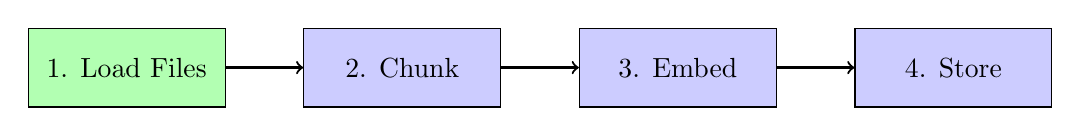
\begin{tikzpicture}[
        box/.style={rectangle, draw, minimum width=2.5cm, minimum height=1cm, fill=blue!20},
        arrow/.style={->, thick}
    ]
        \node[box, fill=green!30] (load) at (0, 0) {1. Load Files};
        \node[box] (chunk) at (3.5, 0) {2. Chunk};
        \node[box] (embed) at (7, 0) {3. Embed};
        \node[box] (store) at (10.5, 0) {4. Store};
        
        \draw[arrow] (load) -- (chunk);
        \draw[arrow] (chunk) -- (embed);
        \draw[arrow] (embed) -- (store);
    \end{tikzpicture}
    
    \vspace{0.5cm}
    
    \textbf{This lab focuses on Step 1: Loading documents!}
    
    \begin{itemize}
        \item Read Markdown files containing disease information
        \item Process text content
        \item Prepare for chunking in Lab 03
    \end{itemize}
\end{frame}

\begin{frame}[fragile]{Opening Files: The with Statement}
    \textbf{Always use \texttt{with} statement - it auto-closes the file!}
    
    \begin{lstlisting}
# Good practice: using 'with'
with open("data/rubella.md", "r", encoding="utf-8") as f:
    content = f.read()

# File is automatically closed after the block
print(content)
    \end{lstlisting}
    
    \vspace{0.3cm}
    
    \textbf{Parameters explained:}
    \begin{itemize}
        \item \texttt{"data/rubella.md"} - file path
        \item \texttt{"r"} - read mode
        \item \texttt{encoding="utf-8"} - supports Thai characters
    \end{itemize}
\end{frame}

\begin{frame}[fragile]{Reading Methods}
    \begin{columns}
        \begin{column}{0.5\textwidth}
            \textbf{read() - Entire file as string}
            \begin{lstlisting}
with open("file.md", "r") as f:
    content = f.read()
    
print(content)
# "Line 1\nLine 2\nLine 3"
            \end{lstlisting}
        \end{column}
        \begin{column}{0.5\textwidth}
            \textbf{readlines() - List of lines}
            \begin{lstlisting}
with open("file.md", "r") as f:
    lines = f.readlines()
    
print(lines)
# ["Line 1\n", "Line 2\n"]
            \end{lstlisting}
        \end{column}
    \end{columns}
    
    \vspace{0.5cm}
    
    \begin{block}{Which to use?}
        \begin{itemize}
            \item \texttt{read()} - when you need the whole content
            \item \texttt{readlines()} - when processing line by line
        \end{itemize}
    \end{block}
\end{frame}

\begin{frame}[fragile]{Counting Characters and Lines}
    \begin{lstlisting}
with open("data/rubella.md", "r", encoding="utf-8") as f:
    content = f.read()

# Count characters
char_count = len(content)
print(f"Characters: {char_count}")

# Count lines
line_count = content.count("\n") + 1
print(f"Lines: {line_count}")

# Or use readlines
with open("data/rubella.md", "r", encoding="utf-8") as f:
    lines = f.readlines()
    print(f"Lines: {len(lines)}")
    \end{lstlisting}
\end{frame}

\begin{frame}[fragile]{Searching Text in Files}
    \begin{lstlisting}
with open("data/rubella.md", "r", encoding="utf-8") as f:
    content = f.read()

# Check if word exists
if "fever" in content:
    print("Found 'fever' in the document!")

# Count occurrences
count = content.count("symptom")
print(f"'symptom' appears {count} times")

# Find lines containing a word
with open("data/rubella.md", "r", encoding="utf-8") as f:
    for line in f:
        if "treatment" in line.lower():
            print(line.strip())
    \end{lstlisting}
\end{frame}

\begin{frame}[fragile]{File Encoding: UTF-8}
    \textbf{UTF-8 encoding is essential for:}
    \begin{itemize}
        \item Thai text
        \item Chinese, Japanese, Korean
        \item Emoji and special characters
    \end{itemize}
    
    \vspace{0.3cm}
    
    \begin{lstlisting}
# Always specify encoding for non-ASCII text
with open("thai_doc.md", "r", encoding="utf-8") as f:
    content = f.read()

# This will contain Thai text correctly
print(content)  # "หัดเยอรมัน คืออะไร..."
    \end{lstlisting}
    
    \begin{alertblock}{Important}
        Without \texttt{encoding="utf-8"}, Thai text may appear as garbage characters!
    \end{alertblock}
\end{frame}

\begin{frame}[fragile]{Complete Example: Document Loader}
    \begin{lstlisting}
def load_document(filepath):
    """Load a document and return its info."""
    with open(filepath, "r", encoding="utf-8") as f:
        content = f.read()
    
    return {
        "filepath": filepath,
        "content": content,
        "char_count": len(content),
        "line_count": content.count("\n") + 1
    }

# Use it
doc = load_document("data/rubella.md")
print(f"File: {doc['filepath']}")
print(f"Characters: {doc['char_count']}")
print(f"Lines: {doc['line_count']}")
    \end{lstlisting}
\end{frame}

\begin{frame}{Summary}
    \begin{columns}
        \begin{column}{0.5\textwidth}
            \textbf{What we learned:}
            \begin{itemize}
                \item \texttt{open()} with \texttt{with} statement
                \item \texttt{read()} vs \texttt{readlines()}
                \item Counting: \texttt{len()}, \texttt{count()}
                \item Searching: \texttt{in}, \texttt{count()}
                \item UTF-8 encoding for Thai
            \end{itemize}
        \end{column}
        \begin{column}{0.45\textwidth}
            \textbf{Connection to RAG:}
            \begin{itemize}
                \item Load documents from files
                \item Next: Chunk the text
                \item Later: Create embeddings
                \item Finally: Store in vector DB
            \end{itemize}
        \end{column}
    \end{columns}
    
    \vspace{0.5cm}
    
    \begin{block}{Next Lab}
        Lab 03: Text Chunking - splitting documents into smaller pieces!
    \end{block}
\end{frame}

\begin{frame}{Exercise Preview (4 exercises, 100 points)}
    \begin{enumerate}
        \item \textbf{Read file content} (25 pts) \\
              Load rubella.md and store content in a variable
        \item \textbf{Count characters} (25 pts) \\
              Count total characters in the file
        \item \textbf{Count lines} (25 pts) \\
              Count total lines in the file
        \item \textbf{Find text} (25 pts) \\
              Count how many times "symptom" appears
    \end{enumerate}
    
    \begin{alertblock}{Time: 45 minutes}
        Work on \texttt{exercise/Lab02\_Exercise.ipynb}
    \end{alertblock}
\end{frame}

\begin{frame}
    \begin{center}
        \Huge \textbf{Questions?}
        
        \vspace{1cm}
        
        \Large Let's start the Tutorial!
        
        \vspace{0.5cm}
        
        \normalsize Open: \texttt{tutorial/Lab02\_Tutorial.ipynb}
    \end{center}
\end{frame}

\end{document}
